
\section{mass continuity}

\begin{frame}{the most basic shallow assumption}

\begin{columns}

\begin{column}{0.6\textwidth}
\begin{itemize}
\item there are many shallow theories: SIA, SSA, hybrids, Blatter, \dots \nocite{Blatter}
\item \emph{all} make one assumption not required in the (non-shallow) Stokes theory:

\begin{center}
\emph{the surface and base of the ice are given by differentiable functions} $z=h(t,x,y)$ \emph{and} $z=b(t,x,y)$
\end{center}
\item surface overhang is not allowed
\end{itemize}
\end{column}

\begin{column}{0.4\textwidth}
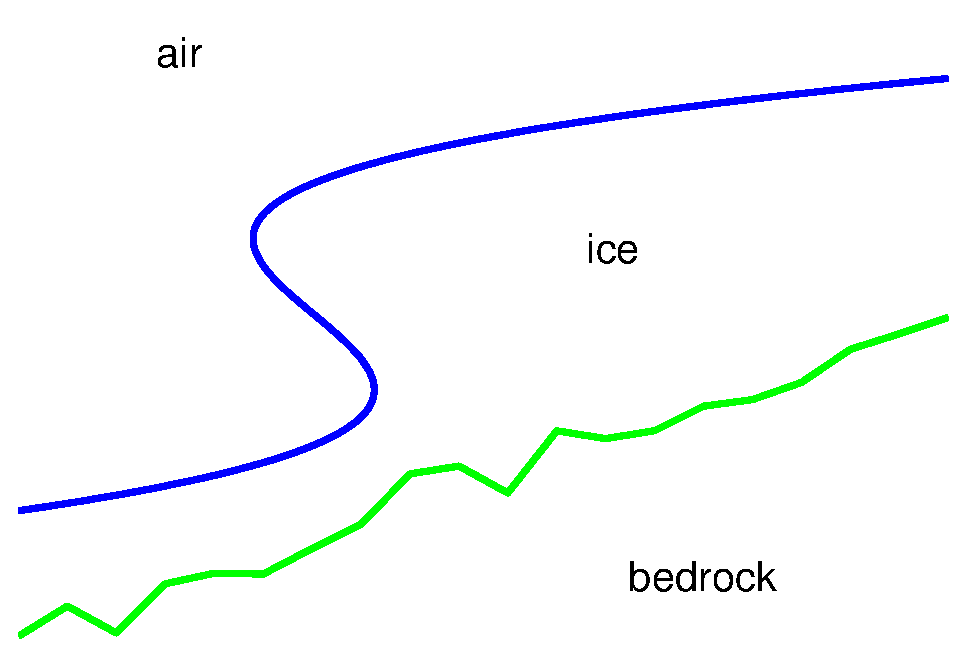
\includegraphics[width=1.0\textwidth]{sshape}

\scriptsize
\begin{center}
\alert{not shallow!}
\end{center}
\vspace{6mm}

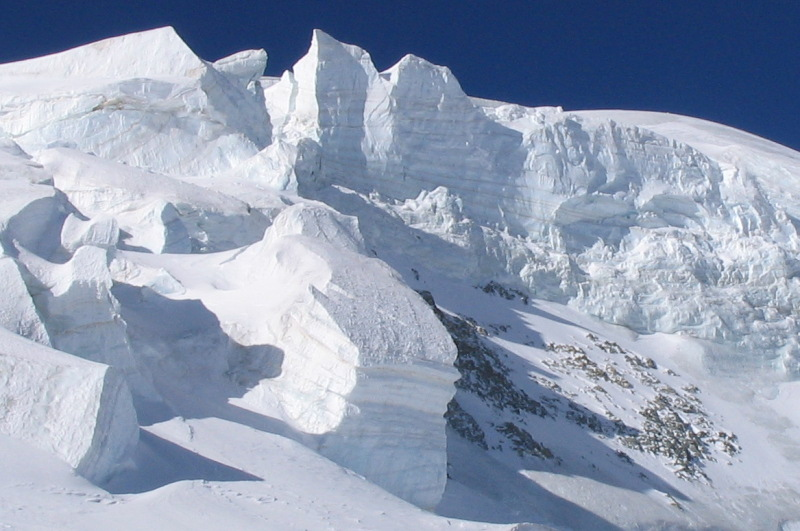
\includegraphics[width=1.0\textwidth]{Serac2}

\begin{center}
\alert{not shallow!}
\end{center}
\end{column}
\end{columns}
\end{frame}


\begin{frame}{kinematic and mass continuity equations}

\begin{itemize}
\item what does this ``most basic shallow assumption'' get you?
\item \emph{answer:} a map-plane mass continuity equation
\item consider these three equations (\emph{on next slide}):
  \begin{itemize}
  \item[$\circ$]  the surface kinematical equation
  \item[$\circ$]  the base kinematical equation
  \item[$\circ$]  the map-plane mass continuity equation
  \end{itemize}
\item under the ``most basic shallow assumption'', 

\begin{center}\emph{any two imply the third}\end{center}
\item you connect the three equations by
  \begin{itemize}
  \item[$\circ$]  the incompressibility of ice
    $$u_x + v_y + w_z = 0$$
  \item[$\circ$]  and the Leibniz rule for differentiating integrals
  \scriptsize
    $$\frac{d}{dx}\left(\int_{g(x)}^{f(x)} h(x,y)\,dy\right) = f'(x) h(x,f(x)) - g'(x) h(x,g(x)) + \int_{g(x)}^{f(x)} h_x(x,y)\,dy$$
  \end{itemize}
\end{itemize}
\end{frame}


\begin{frame}{kinematic and mass continuity equations 2}

\begin{itemize}
\item let $a$ be the surface mass balance function ($a>0$ is accumulation), and
\item $s$ be the basal melt rate function ($s>0$ is basal melting), so
\item $M=a-s$
\item define the map-plane flux of ice,
	$$\bq = \int_{b}^{h} (u,v)\,dz = \overline{\mathbf{u}}\,H$$
\item the three equations are:
\begin{empheq}[left=\text{surface kinematical}\quad,innerbox=\fbox]{equation}
h_t = a - u\big|_h h_x - v\big|_h h_y + w\big|_h  \label{surfkine}
\end{empheq}
\begin{empheq}[left=\text{base kinematical}\quad,innerbox=\fbox]{equation}
b_t = s - u\big|_b b_x - v\big|_b b_y + w\big|_b  \label{basekine}
\end{empheq}
\begin{empheq}[left=\text{mass continuity}\qquad\qquad\quad,innerbox=\fbox]{equation}
H_t = M - \Div \bq \label{masscontinuity}
\end{empheq}
\end{itemize}
\end{frame}


\begin{frame}{kinematic and mass continuity equations 3}

\begin{itemize}
\item literature is full of incomplete calculations of these shallow equivalences
\item \dots usually mixed in with small-parameter arguments about shallow stress balances
\item most ice sheet models use the mass continuity equation to describe change in ice sheet geometry
\item \dots but they could instead use the surface kinematical equation
\end{itemize}
\end{frame}


\begin{frame}{standard recipe for ice sheet models}

\begin{itemize}
\item the ingredients of a typical ice sheet model:
  \begin{enumerate}
  \item numerical implementation of a stress balance: gives velocity $(u,v,w)$
  \item from the horizontal velocity $(u,v)$ and the surface balance, do time-step of mass continuity equation to get $H_t$
  \item update upper and lower surface elevation
  \item decide on time-step, and repeat at 1.
  \end{enumerate}
\end{itemize}
\end{frame}
